\section{Marco teórico}

\subsection{Eliminación Gaussiana}
\label{sec:gaussiana}

Los sistemas de ecuaciones lineales pueden ser representados en forma matricial como \textit{Ax=b}, donde A representa la matriz de los coeficientes que acompañan a cada una de las incógnitas, \textit{x} representa al vector de incógnitas y \textit{b} al vector de términos independientes. Para los sistemas cuadrados, donde hay misma cantidad de incógnitas que de ecuaciones, el método de eliminación Gaussiana busca darle valor a los coeficientes del vector de incógnitas y resolver el sistema lineal. El modelado de sistemas de ecuaciones con matrices se extiende a una amplia gama de disciplinas como los gráficos por computadora, las finanzas y las ingenierías, entre otras, las cuales no serían como las conocemos sin este objeto y las operaciones que podemos hacer con él. 

\begin{figure}[h]
    \centering
    \begin{minipage}{0.3\linewidth}
        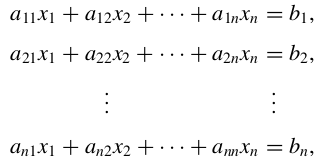
\includegraphics[width=\linewidth]{img/sistema_de_ecuaciones.png}
        \caption{Un sistema de ecuaciones}
    \end{minipage}
  \begin{minipage}{0.45\linewidth}
      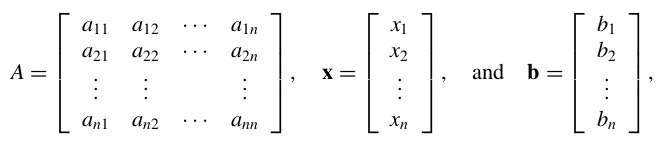
\includegraphics[width=\linewidth]{img/combinacion_lineal.png}
      \caption{Su forma matricial}
  \end{minipage}
  \caption{Sistemas de ecuaciones con su respectiva representación matricial}
\end{figure}

El proceso para resolver mediante este método comienza con la matriz original y se va aplicando sobre ella una serie de pasos hasta obtener una matriz de forma triangular superior. Para realizar esto, se recorre cada elemento $a_{ii}$ perteneciente a la diagonal principal, poniendo en ceros los elementos debajo de éste; este proceso se llama diagonalización. Una vez diagonalizado el sistema, buscamos darle valores a los coeficientes del vector de incógnitas por medio de un despeje desde abajo hacia arriba, es decir, empezamos por el coeficiente inferior del vector $x$ y subiendo por el mismo usando los valores despejados previamente para obtener nuevas soluciones para los próximos coeficientes. Éste  método descripto se conoce como \textit{Gaussian elimination with Backward substitution} \cite{Burden11}.
Considerando lo anterior, podemos notar que resolver el sistema de ecuaciones tiene una complejidad computacional de $\mathcal{O}(n^3)$.

\subsection{Métodos de pivoteo para diagonalización}
\label{sec:pivoteo}

Para casos donde encontramos, o  ``creamos'' por medio del mismo proceso de diagonalización, un cero en la diagonal de la matriz existen formas de obtener versiones equivalentes del sistema donde podemos continuar nuestro algoritmo de eliminación Gaussiana. Estos métodos se llaman \textit{pivoteos parciales o totales} y constan en hacer intercambios de filas o de columnas para que el sistema pueda seguir soportando el algoritmo. Cuando los intercambios son de filas los llamamos pivoteos parciales y cuando lo son de filas y columnas los llamamos pivotes totales. En el presente trabajo nos centraremos en pivoteos parciales. Observese en la figura \ref{fig:pivoting} como el proceso de eliminación gaussiana puede solucionar el hecho de encontrar un cero en la diagonal por medio del intercambio de filas.

\begin{figure}[H]
    $$
    \left[\begin{array}{cccc|c}
    2 & 2 & -1 & 3 & 13 \\
    -2 & -2 & 0 & 0 & -2 \\
    4 & -1 & -2 & 4 & 24 \\
    -6 & -2 & 2 & -3 & -10
    \end{array}\right] \rightarrow \begin{gathered}
    F_2-(-1) F_1 \\
    F_3-(2) F_1 \\
    F_4-(-3) F_1
    \end{gathered} \longrightarrow\left[\begin{array}{cccc|c}
    2 & 2 & -1 & 3 & 13 \\
    0 & \textbf{0} & -1 & 3 & 11 \\
    0 & -5 & 0 & -2 & -2 \\
    0 & 0 & -1 & 6 & 29
    \end{array}\right]\longrightarrow\left[\begin{array}{cccc|c}
    2 & 2 & -1 & 3 & 13 \\
    0 & -5 & 0 & -2 & -2 \\
    0 & 0 & -1 & 3 & 11 \\
    0 & 0 & -1 & 6 & 29
    \end{array}\right]
    $$
    
    \caption{El sistema de ecuaciones se encuentra con un cero en la diagonal luego del primer paso del algoritmo y debemos aplicar un intercambio entre la segunda y la tercer fila para poder continuar la diagonalización.}
    \label{fig:pivoting}

\end{figure}

\subsubsection{¿Todo sistema de ecuaciones se puede diagonalizar?}
\label{sec:sin_solucion}

Si una matriz es singular no tenga inversa. Esto ocurre cuando alguna fila de la matriz puede expresarse como combinación lineal de las otras filas. Por ejemplo, dada la siguiente matriz:

\begin{center}
$\begin{bmatrix}
1 & -1 & 3\\
-2 & 2 & -6\\
1 & 5 & 7
\end{bmatrix}$
\end{center}

La triangulación da como resultado la siguiente matriz:

\begin{center}
$\begin{bmatrix}
1 & 2 & 3\\
0 & 0 & 0\\
0 & 1 & 2
\end{bmatrix}$
\end{center}

Esta ecuación solo tiene resultado cuando b$_2$ es igual a 0. En ese caso tiene infinitas soluciones. Caso contrario, no existe solución.

Por este motivo no todo sistema de ecuaciones se puede diagonalizar y esto no importa el algoritmo que usemos.

\iffalse
Otro ejemplo, es tener una matriz tal que la primera columna tenga todos sus elementos iguales a 0. El problema aquí es que el primer elemento de la diagonal principal (posición [0,0]) es 0, lo que significa que no se puede usar como pivote.

\begin{center}
$\begin{bmatrix}
0 & 1 & -1 & 3\\
0 & -0.5 & 0 & 0\\
0 & 1 & -2 & 4\\
0 & -1 & 2 & -3
\end{bmatrix}$
\end{center}

\fi


\subsection{Matriz inversa: relaci´ón con la diagonalizaci´ón}
\label{opcionales}
\label{sec:inversa}

La matriz inversa de una matriz $A$, la cual denotaremos como $A^{-1}$, es una matriz que cumple con la propiedad de $A.A^{-1}=A^{-1}.A=I$ siendo $I$ la matriz identidad. Esta matriz inversa no siempre existe. Si la matriz $A$ cumple ser cuadrada y que su determinante \cite{Strang-determinante} sea distinto de cero, entonces esta matriz si existe.

Nuestro objetivo entonces, es calcular la matriz inversa de una matriz A utilizando el método de eliminación gaussiana (EG) con una matriz aumentada (figura \ref{fig:aumentada}). Este enfoque se basa en transformar la matriz A en su forma diagonal, y al mismo tiempo, aplicar las mismas operaciones a la matriz identidad para obtener la inversa de A.

El proceso consiste en construir una matriz aumentada que combine A y la matriz identidad I. Luego, mediante la eliminación gaussiana, se van realizando operaciones fila por fila para convertir A en la matriz identidad. Al final de este proceso, la matriz que acompaña a I será la inversa de A. Se puede ver un ejemplo de como se calcula la inversa en la figura (\ref{fig:jordan_ejemplo}). En la misma se puede apreciar cada paso como lo explicamos reci´én.

\begin{figure}[]
    \centering
    \begin{minipage}{0.15\linewidth}
        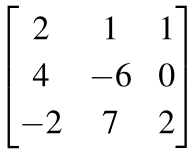
\includegraphics[width=\linewidth]{img/matriz-a-aumentar.png}
        \caption{Matriz A}
    \end{minipage}
  \begin{minipage}{0.3\linewidth}
      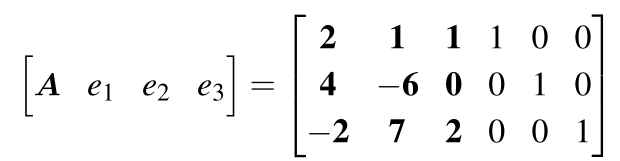
\includegraphics[width=\linewidth]{img/matriz-aumentada.png}
      \caption{Matriz ya aumentada}
  \end{minipage}
  \caption{Proceso de aumentar la matriz A.}
  \label{fig:aumentada}
\end{figure}

Este método es una aplicación práctica del algoritmo de Gauss-Jordan y es especialmente útil porque, a diferencia de otras técnicas, no requiere descomposición LU o factorizaciones complicadas. Lo que hacemos es simplemente aplicar operaciones de fila que son fáciles de implementar.

\begin{figure}[]
    \centering
    \begin{minipage}{0.3\linewidth}
        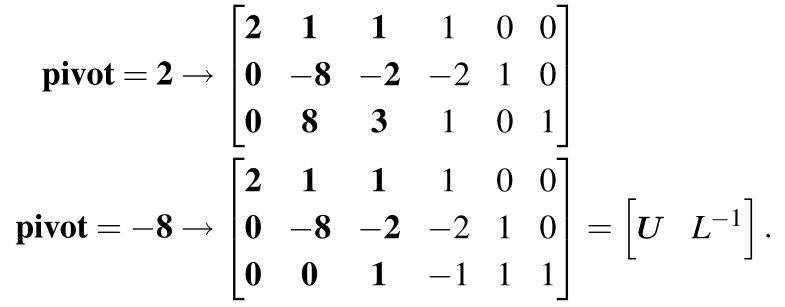
\includegraphics[width=\linewidth]{img/inversa_1.png}
        \caption{Triangular A}
    \end{minipage}
  \begin{minipage}{0.3\linewidth}
      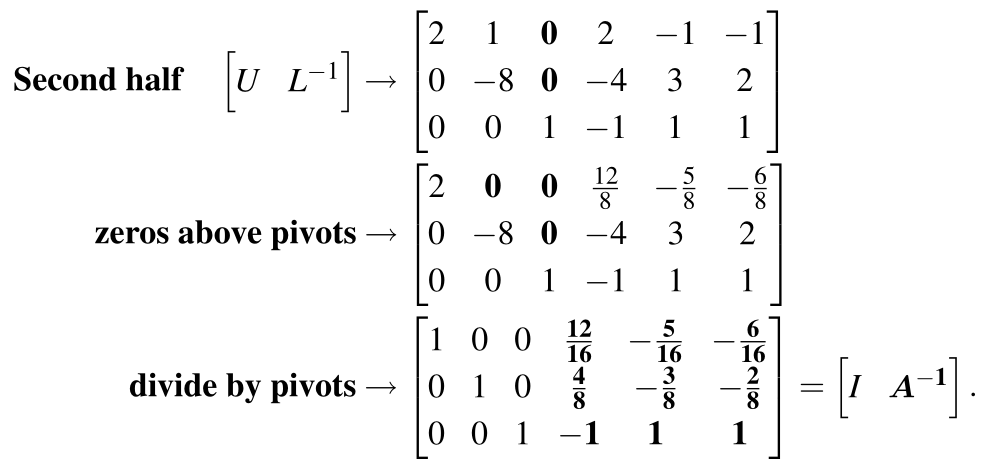
\includegraphics[width=\linewidth]{img/inversa_2.png}
      \caption{Convertir A en la identidad}
  \end{minipage}
  \caption{Ejemplo del algoritmo de Jordan para la matriz A.}
  \label{fig:jordan_ejemplo}
\end{figure}



\subsection{Sistemas tridiagonales}
\label{sec:tridiagonal}

Por su parte, las matrices tridiagonales, caracterizadas por su estructura rala, es decir, sus elementos son solo distintos de cero en la diagonal principal y en las diagonales adyacentes por encima y por debajo de esta, poseen propiedades que permiten operar con ellas con mayor eficiencia que con matrices genéricas. Para estos sistemas tridiagonales, se propone una implementación del algoritmo que reduce el número de operaciones aritméticas de $\mathcal{O}(n^3)$ a $\mathcal{O}(n)$. Esta optimización se consigue al aprovechar la estructura rala de la matriz, evitando cálculos redundantes sobre elementos nulos. Estos sistemas son estudiados en la bibliografía \cite{Recipes07} para dar soluciones eficientes al sistema tratando a cada una de las diagonales como vectores, como también a las incógnitas y a los términos independientes. Para comprender como es la estructura de los mismo puede ver en la figura \ref{fig:tridiagonal} donde logrará observar los vectores c, b, a, d y x los cuales son diagonal superior, diagonal principal, diagonal inferior, término independiente e incognitas respectivamente.  

\begin{figure}[h]

    \[ \begin{bmatrix}
b_1 & c_1 & & & 0\\
a_2 & b_2 & c_2 & & & \\
    & a_3 & b_3 & \ddots & \\
    &    & \ddots &  \ddots&c_{n-1}\\
0   &    &   & a_n & b_n
     \end{bmatrix}
  \begin{bmatrix}
        x_{1}\\
        x_{2} \\
        x_{3}\\ 
        \vdots\\ 
        x_{n}  
 \end{bmatrix}
 =
 \begin{bmatrix}
     d_{1} \\
     d_{2} \\
     d_{3} \\
     \vdots \\
     d_{n} \\
 \end{bmatrix}
 \]
 
 \caption{Estructura de un sistema tridiagonal.}
 \label{fig:tridiagonal}
\end{figure}

\subsection{Operador Laplaciano}
\label{Intro_laplaciano}
\label{sec:laplaciano}

El operador de Laplace o Laplaciano ($\nabla^{2}$) sobre funciones escalares es el diferencial para la divergencia del gradiente. Esto nos da una noción del comportamiento de la función que es utilizada para numerosos procesos físicos, como por ejemplo propagación de ondas o de calor \cite{laplaciano_web}. Este operador también lo podemos usar para problemas de difusión del estilo de caminatas aleatorias \cite{random_walk}

\subsection{Difusión}
\label{Intro_difusion}

 La difusión es un proceso estocástico cuyo modelado implica simular cómo una entidad, en este caso vista como calor, se distribuye en un medio. La ecuación de difusión, que describe este fenómeno, puede ser discretizada y resuelta mediante métodos numéricos. En particular, el operador Laplaciano (sic. \ref{sec:laplaciano}) es un operador diferencial que juega un papel central en la descripción de la difusión. En una dimensión, la versión discreta del Laplaciano es equivalente a la segunda derivada, y se utiliza en varias areas como en el procesamiento de imágenes y análisis de datos en redes.


\subsection{Operador Laplaciano 2D}
\label{Intro_laplaciano2D}
El operador laplaciano discreto en 2D es fundamental para modelar fenómenos como la difusión y el flujo de calor en una malla o grilla de puntos. Este operador se define generalmente como la suma de las diferencias de valores en los puntos vecinos, lo que permite calcular cómo cambia una cantidad en un punto respecto a sus alrededores.

\subsection{Difusión 2D}
\label{Intro_difusion2D}
 La difusión en dos dimensiones (2D) ofrece una perspectiva más compleja en comparación con la difusión unidimensional, ya que ésta permite modelar procesos como la propagación de calor, la dispersión de contaminantes y la dinámica de poblaciones. Utilizando el laplaciano discreto, vamos a establecer ecuaciones que simulan el proceso de difusión.